I dette kapitel vil den initierende problemstilling blive analyseret. Dette bliver gjort i form af en interessentanalyse, hvor de væsentlige interessenter bliver fundet. På baggrund af interessentanalysen blev der sendt et spørgeskema ud, og et interview blev foretaget med VisitAalborg. Til sidst i dette kapitel er to eksisterende løsninger blevet analyseret. 

\section{Interessentanalyse}
Gruppen vil i dette afsnit undersøge diverse personer/grupper, der kan fungere som interessenter i projektet, altså en person der vil have nytte af eller kan bidrage til projektet. Herefter vil gruppen prioritere disse interessenter, alt efter hvor relevante de er i forhold til projektet.

\textbf{Turister}\newline
Turister er en væsentlig interessent i projektet, da en turist ofte vil se hvad byen har at byde på, eller nogle unikke attraktioner, i forhold til følgende citat: \newline 
\textit{“If you want visitors to come back again — and say nice things about your town to others who might come, too — you need to have some good answers at the ready. That means offering things to see and do that are either unique or extraordinary…”} \citep{UniversityOfMinnesota}.\newline 
Hvis turisterne planlægger hvad det er de vil se, kan turisterne spare tid \citep{YouthCentral}. Turisterne kan vælge at gå en længere rute, og derved have mulighed for at finde andre ting, som de vælger at bruge deres tid på. Et ruteplanlægningsværktøj vil derfor være interessant for turister, da de derved kan komme til at besøge alle de attraktioner/seværdigheder, som de ønsker.
En-dagsturister er en mindre interessent i projektet, da en en-dagsturist maksimum overnatter en nat, og generelt har et planlagt formål med rejsen, som fx at besøge Storcenteret, venner/familie eller er på et kursusophold \citep{Faxe}.

\textbf{Erhvervs- og Vækstministeriet}\newline
Erhvervs- og Vækstministeriet (EVM) er en interessent i projektet, da det er dette ministerie, turisme indgår under, da turismen er et erhverv der beskæftiger mange tusinde mennesker. Hvis der er nogle unikke eller ekstraordinære attraktioner i en by, vil turister huske disse, som gode oplevelser, og nogle vil derfor komme igen. Det er noget som EVM er interesseret i, da der kommer flere penge ind i landet \citep{EVM}.
http://www.evm.dk/arbejdsomraader/internationalt-udsyn/turisme
Her vil et ruteplanlægningsværktøj kunne hjælpe turister med at se nogle attraktioner, hvis der fx er en top 5 over de attraktionerne der er i landet, eller i den by ferien foregår.

\textbf{Retail-handel}\newline
Diverse forretninger er også interessenter i projektet, da kendte brands som fx IKEA, Bilka og lignende er så store, at de kan tiltrække turister \citep{PengeloseButikker}. Ved at implementere disse adresser i et ruteplanlægningsværktøj, kan det tiltrække turister, og derved øge omsætningen, til gavn for forretningerne.

\textbf{VisitAalborg}\newline
VisitAalborgs arbejde består af at støtte aktører, hvis disse aktører byder på nogle turistfremmende aktiviteter/projekter, der har til formål at hjælpe Aalborg. Det kan fx være at henvise til aktørernes hjemmesider, gennem deres egen hjemmeside, der bliver set af ca. 600.000 årligt. \citep{VA}
Til et ruteplanlægningsværktøj er VisitAalborg en vigtig interessent, da de har informationer om turisterne i Aalborg. Ved at inddrage turistkontoret i projektet, vil gruppen gøre brug af deres ressourcer. 

\subsection{Prioriteringen}
For at prioritere interessenterne i projektet, og finde de vigtigste interessenter, har gruppen valgt at gøre brug af indflydelse/medvirken-matrixen, som kan ses på figur 2.1 herunder.

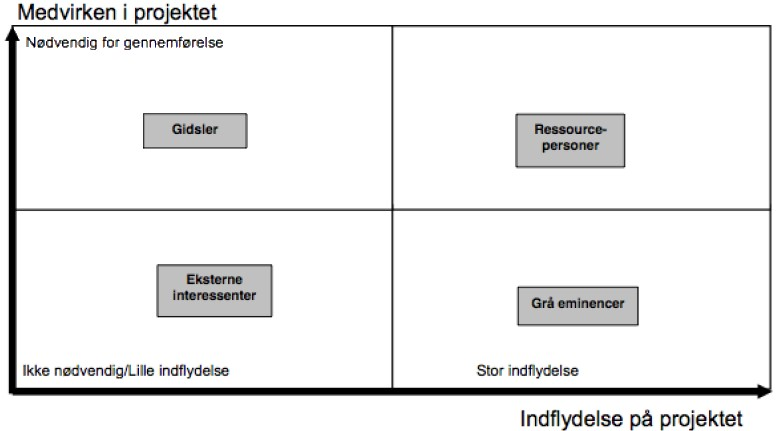
\includegraphics[scale=0.8]{Prior}
\textit{Figur 2.1: Indflydelse/medvirken-matrixen}\newline

Indflydelse/medvirken-matrixen opdeler interessenterne i fire grupper, og giver gruppen et overblik over, hvilke interessenter der skal tages højde for, og hvem der kan bidrage med vigtig information og ressourcer til projektet.

VisitAalborg er i dette projekt ressourceperson, da de har informationer om turisme. Derudover kan turistkontoret komme med råd og vejledning for, at en eventuel løsning vil være mest optimal for turisterne.   \newline
Turisterne er også kategoriseret som ressourceperson, da turisternes viden og erfaringer fra deres storbyferier, kan bruges til projektet.

De eksterne i projektet er retail-forretningerne og Erhvervs- og Vækstministeriet. Deres indflydelse og medvirken er ikke nødvendig, for at kunne gennemføre projektet, men projektet kan stadig have en indflydelse på dem.

Gruppen har i dette projekt ikke nogle interessenter, der passer ind under kategorierne grå eminence og gidsler.

\subsection{Opsummering}
Ud fra interessentanalysen, er gruppen nået frem til, at VisitAalborg og turisterne er ressourcepersoner, hvilket gruppen ser som en centrale interessenter i projektet. Det er nødvendige kilder, for at få nogle brugbare ressourcer.
De andre interessenter, som gruppen har fundet frem til, er blevet vurderet som mindre vigtige, og derfor vil fokusset ligge hos VisitAalborg og turisterne.
Da turister og turistbureauet er projektets væsentligste interessenter, har gruppen valgt at uddrage information fra disse to interessenter i form af et spørgeskema og et interview. 
I tilfælde af VisitAalborg og turisternes interesser modstrides, vil gruppen vægte turisternes interesser højest, da VisitAalborg kan have økonomiske interesser i at fremme bestemte partnere, fx Aalborg Zoo, Nordkraft og Aalborg Kongress og Kulturcenter \citep{VA}. 

Det kommende afsnit vil omhandle informationsøgning, i form af det udsendte spørgeskema. 


